% Section 5.2 (Visual Breakdown & Observations)

\subsubsection{Visualizing Empirical Trade-Offs and Key Observations}
\label{sec:results_interp}

Figures~\ref{fig:overview}--\ref{fig:tokens} dissect the empirical profile across all four experimental conditions (\textbf{E1}--\textbf{E4}, 128 runs total) by aggregate split metrics, difficulty scaling, Stage~3 formal outcomes, and generation efficiency.

\begin{figure}[htbp]
  \centering
  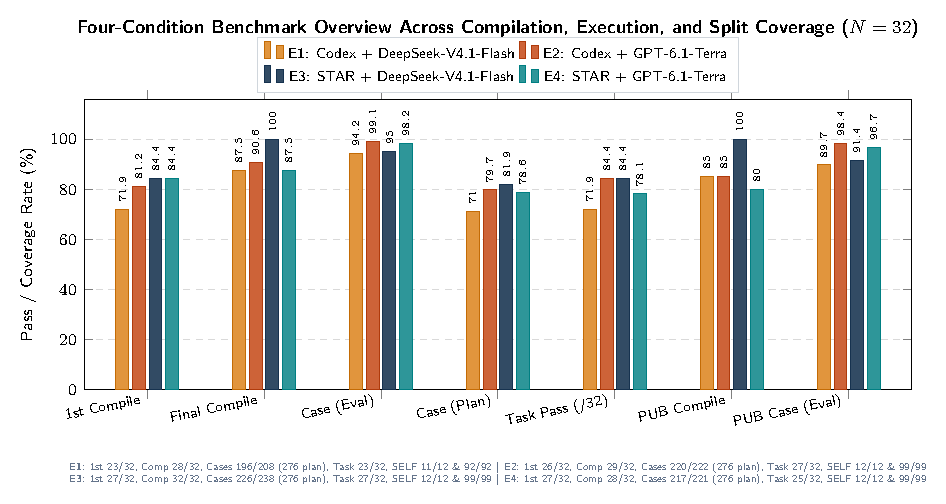
\includegraphics[width=0.98\textwidth]{fig2_four_group_overview.pdf}
  \caption{Cross-condition comparison across \textbf{E1} (Codex + DeepSeek), \textbf{E2} (Codex + Terra), \textbf{E3} (STAR + DeepSeek), and \textbf{E4} (STAR + Terra) covering first-pass and final compilation, evaluated vs.\ planned fixed cases, task-level pass rate, and \code{public} ($n=20$) vs.\ \code{self_built} ($n=12$) splits.}
  \label{fig:overview}
\end{figure}

\begin{figure}[htbp]
  \centering
  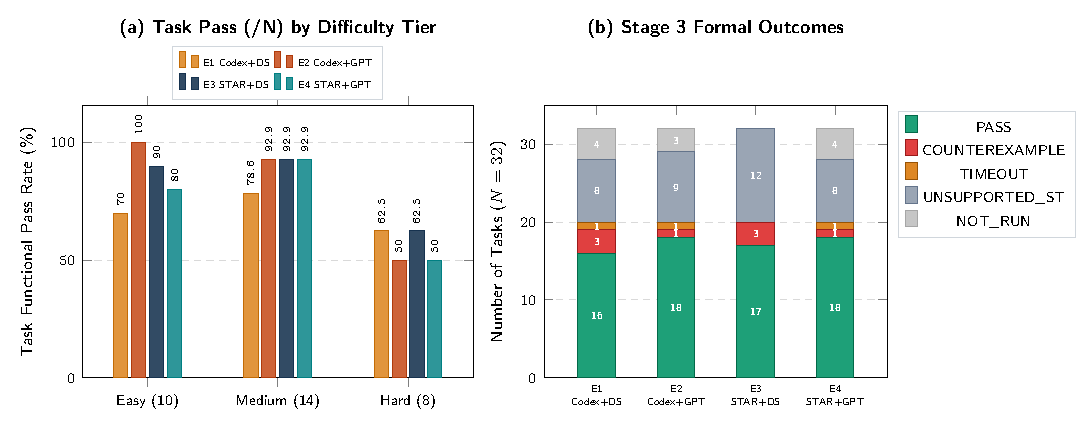
\includegraphics[width=0.98\textwidth]{fig3_difficulty_formal_breakdown.pdf}
  \caption{Stratified performance and formal diagnosis across \textbf{E1}--\textbf{E4}: (a)~task-level functional pass rate across Easy ($n=10$), Medium ($n=14$), and Hard ($n=8$) tiers; (b)~Stage~3 formal \code{ST->SMV} outcome counts ($N=32$ tasks per condition).}
  \label{fig:breakdown}
\end{figure}

\begin{figure}[htbp]
  \centering
  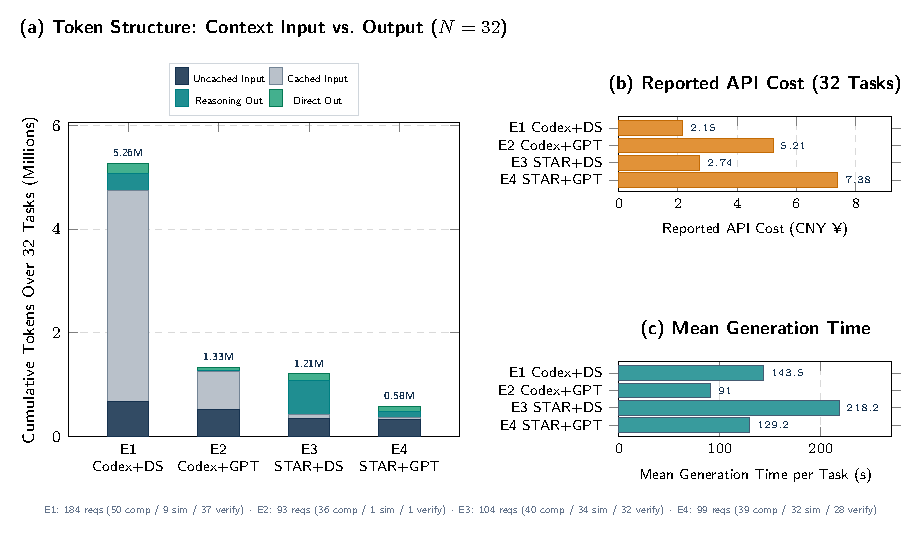
\includegraphics[width=0.96\textwidth]{fig4_token_cost_efficiency.pdf}
  \caption{Generation resource efficiency across \textbf{E1}--\textbf{E4} ($N=32$ tasks per condition): (a)~cumulative 32-task input tokens (cached vs.\ uncached) and output tokens (reasoning vs.\ direct emission); (b)~total reported provider API cost (RMB); (c)~mean generation elapsed time per task (s).}
  \label{fig:tokens}
\end{figure}

Four consistent empirical findings emerge from Table~\ref{tab:benchmark} and Figures~\ref{fig:overview}--\ref{fig:tokens}:
\begin{enumerate}
  \item \textbf{Framework Benefit Depends Sharply on Foundation Model Capability (\textbf{E3} vs.\ \textbf{E1})}: On \code{deepseek-v4.1-flash-1017}, unguided \code{Codex CLI} (\textbf{E1}) issues 184 LLM requests and 50 compiles, accumulating 4,742,114 input tokens (4,057,344 cached, 684,770 uncached) across multi-turn agent transcripts, yet stalls at \textbf{28/32 (87.5\%)} compilation, 196/208 (94.2\% evaluated; 71.0\% planned) fixed cases, and 23/32 (71.9\%) task passes with 10 functional failures. Under \textbf{STAR} (\textbf{E3}), view isolation, targeted dialect cards, and compact diagnostics raise compilation to \textbf{32/32 (100.0\%)}, lift evaluated cases to 226/238 (and peak planned coverage at \textbf{81.9\%}), boost task passes to 27/32 (halving \code{FAIL} outcomes to 5), and compress total input volume roughly \textbf{11$\times$} to 432,953 tokens (104 requests).
  \item \textbf{Structured Multi-Role Pipeline vs.\ Unconstrained Tool-Use on Stronger Models (\textbf{E2} vs.\ \textbf{E4})}: On \code{gpt-6.1-terra}, unconstrained \code{Codex CLI} (\textbf{E2}) rarely requires exploratory recovery (triggering only 1 in-loop simulation and 1 formal call across all 32 tasks), achieving \textbf{29/32 (90.6\%)} compilation, the matrix-high \textbf{99.1\% (220/222)} evaluated case pass rate, and \textbf{27/32} task passes (27/29 = 93.1\% evaluated) with minimal 72,823 total output tokens, \textyen 5.21 cost, and 91.0\,s mean generation latency. Under \textbf{STAR} (\textbf{E4}), the model achieves the same \textbf{18} Stage~3 formal \code{PASS} verdicts and lowest input footprint (365,578 tokens), but mandatory multi-stage JSON Planning, Coding, and Testing inflate total output tokens nearly $3\times$ (215,832), raising cost to \textyen 7.38 and mean latency to 129.2\,s while passing two fewer tasks overall (one extra \code{FAIL} on \code{PUB004} and one extra lock timeout on \code{PUB006}). Fixed heavy orchestration therefore adds output overhead on models already strong enough to compile cleanly, motivating adaptive difficulty-gated routing.
  \item \textbf{High Reliability on Self-Built Control Suite (\code{SELF001}--\code{SELF012})}: Across \textbf{E2}, \textbf{E3}, and \textbf{E4}, all three conditions achieve \textbf{12/12 compilation, 99/99 fixed-case pass, and 12/12 Stage~3 formal verification pass}. Across all 48 self-built runs in the $2 \times 2$ matrix, only one run failed---\textbf{E1}/\code{SELF009}---solely due to omitting CODESYS static-analysis dialect guardrails (\code{SA0027}).
  \item \textbf{Lock Contention Dominates GPT Compilation Gaps and \code{PARTIAL} Bounds Reflect Execution Scope}: Beyond \code{PUB018} (\code{VARIANT} reflection), all uncompiled tasks in \textbf{E2} (\code{PUB014}, \code{PUB017}) and \textbf{E4} (\code{PUB006}, \code{PUB014}, \code{PUB017}) terminated as infrastructure \code{TOOL_ERROR}s from compiler mutex contention (\code{Compiler lock wait deadline exceeded}), directly prompting commit \pathcode{cef1388} to decouple lock wait deadlines from compile timeouts. Separately, \code{PARTIAL} verdicts in \pathcode{batch.py} stem from physical hour-scale timer exclusions and explicit \code{UNSUPPORTED_ST} lowering exits rather than silent falsification.
\end{enumerate}